\subsection{Universal Covering of $\E_2$}

In this section, we want to establish an operadic structure on the sequence of
universal coverings of $\E_2$ of each degree. We recall the operad $\E_2$ from
Example \ref{eg:operads} which we introduced as the little 2-disks operad. So in
each configuration space $\E_2(n)$ we have $n$ disks embedded into a large disk
by translation and resizing such that the images of the embedding do not intersect. We use topological
terms when talking about $\E_2$. What really happens is that we apply them
level-wise. We see that $\widetilde{E_2}(n)$, the universal coverings of $\E_2(n)$ for all $n \in \N$,
can be equipped with an operadic structure as well as a braid action. 
We state and sketch results from \cite{fox}, as it is the key factor to establish a braid action.
Hence, we
obtain another example of a braided operad.
Note that later there is an alternative construction of $\widetilde{E_2}$ via Example \ref{eg:br-fib-trivial}
applied to the trivial braided operad.


The operadic structure of $\E_2$ requires each configuration to have labels as they are necessary to define the
composition maps. However, the images of the disk embeddings of configurations that only
differ in their labels are identical. 
Therefore, consider the quotient
under the symmetric group action for all $n \in \N$:
\[
    \E_2(n) \to \E_2(n) \slash S_n,
\]
which we call the unordered little disk space.
We denote the family of these quotient spaces by $\E_2 \slash S$. Note that this is not
an operad any longer as the composition map requires labels. 


The following lemma is essential to establish a braid group action on 
the universal covering $\widetilde{\E_2}(n)$.

\begin{lem}\label{lem:fundamentalgroup} The following statements hold for every
    configuration $\E_2(n)$ for all $n \in \N$:
    \begin{enumerate}
        \item The fundamental group of the space of little disks $\E_2(n)$ is the pure braid group $PB_n$.
        \item The fundamental group of the unordered little disks space $\E_2(n) \slash S_n$ is the braid
        group $B_n$.
    \end{enumerate}
\end{lem}

We do not prove the
lemma here. A proof by Fox and Neuwirth can be found in \cite{fox}. However, we
give a sketch of why this is the case at the end of the section.

Before we get started, we need to define what it means to be a universal
covering of a topological operad.

\begin{defin}
    Let $\P$  be a topological operad. A \emph{covering operad} $\widetilde{\P}$ is a
    topological operad such that there is a morphism of operads $c \colon
    \widetilde{\P} \to \P$ where $c_n \colon \widetilde{\P}(n) \to \P(n)$ is a
    covering of $\P(n)$ for all $n \geq 1$.
\end{defin}

\begin{defin}
    Let $\P$ be a topological operad. A \emph{universal covering operad}
    $\widetilde{\P}$ is a covering operad that is universal in every degree $n
    \geq 1$.
\end{defin}

To be able to talk about universal covers and fundamental groups
we need to choose a basepoint. So formally, for any choice of a basepoint on
each level $n$, permuting its labels gives us a different point in
$\E_2(n)$. Hence, if we consider a loop at a basepoint we are required to end
the loop with the same labeling of the configuration of the basepoint.
That is the reason why when considering the fundamental group of $\E_2(n)$ over some basepoint, we
only obtain the pure braid group on $n$ strands by Lemma
\ref{lem:fundamentalgroup}. 
In this section we want to establish a universal
covering of $\E_2$ which has the full braid action. 
In the next step, we first define a universal covering of $\E_2$ and $\E_2 \slash S$ for each level $n$.
Then, we see that these spaces are homeomorphic on each level. This allows us to transfer the braid action on
the universal covering of $E_2 \slash S$ to the universal covering of
$\E_2$.

In this part,
we work a lot with $\Ex$ which is constructed from $\E_2$ using Definition \ref{def:Ox}. This gives us a nice way to talk about configurations and paths between
them. Hence, let us recall the definition of $\Ex$:
\begin{rem}\label{rem:ex}
    The objects of $\Ex$ are the finite pointed sets $\langle n \rangle$ for all
    $n \in \N$. A morphism $\langle n \rangle \to \langle m \rangle$ in $\Ex$
    consists of a morphism $\alpha \colon \langle n \rangle \to \langle m
    \rangle$ in $\Fin$ and a collection of configurations
    $$\{c_j \in \E_2(|\alpha^{-1}(j)|)\}_{1 \leq j \leq m},$$ where each
    configuration is labeled by $\alpha^{-1}(j)$.

    We denote the trivial configuration with label $x$ by $\id^{(x)} \in \E_2(1)$.
    For $\sigma \in S_n$, we refer to the corresponding automorphism of $\langle
    n \rangle$ with configurations $(\id^{(1)}, \dots, \id^{(n)})$ also by $\sigma$.
    Further, recall the composition in $\Ex$. Let 
    \begin{center}
        $\alpha \colon \langle n \rangle \to \langle m \rangle$ with
        configurations $\{c_j\}_{1 \leq j \leq m}$ 
    \end{center}
    and 
    \begin{center}
        $\alpha' \colon \langle m \rangle \to \langle l \rangle$ with
        configurations $\{c'_k\}_{1 \leq k \leq l}$,
    \end{center}
    Then, the configuration $c'_k$ is labeled by $\alpha'^{-1}=\left\{j_1^{(k)},
    \dots, j_p^{(k)}\right\}$. Thus, with the composition map $\gamma$ we obtain a configuration 
    \[
        \gamma(c'_k, c_{j_1}, \dots, c_{j_p})
    \]
    labeled by $(\alpha' \circ \alpha)^{-1}(k)$ for all $1 \leq k \leq l$ giving
    us the well-defined composition $\alpha' \circ \alpha$.
\end{rem}

\begin{eg}
    An example of a morphism in $\Ex$ is the following:
    \begin{align*}
        \alpha \colon \langle 3 \rangle &\to \langle 2 \rangle \\ 1 &\mapsto 1 \\
        2 &\mapsto 2 \\
        3 &\mapsto 1 \\
    \end{align*}
    together with the configurations:
    \begin{center}
    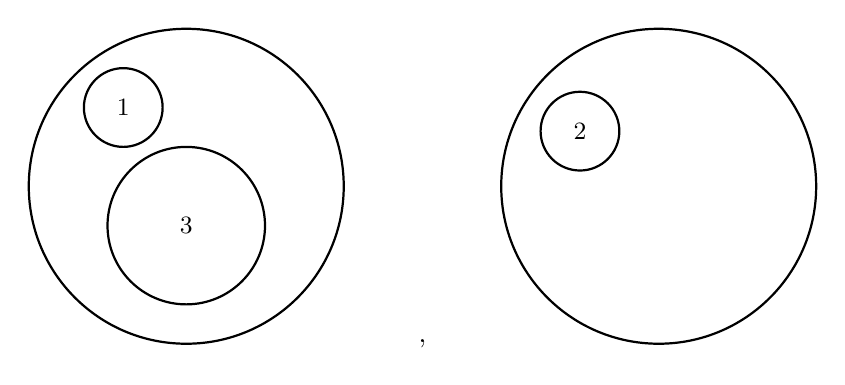
\begin{tikzpicture}
                        % First element (left)
                        \draw[thick] (-3,0) circle (2); \draw[thick] (-3.8, 1)
                        circle (0.5); \draw[thick] (-3, -0.5) circle (1); \node
                        at (-3.8, 1) {\small $1$}; \node at (-3, -0.5) {\small
                        $3$}; \node at (0,-2) {,};
                        % Second element (right)
                        \draw[thick] (3,0) circle (2); \draw[thick] (2,0.7)
                        circle (0.5); \node at (2,0.7) {\small $2$};
        \end{tikzpicture}
    \end{center}
\end{eg}
The category $\Ex$ is an essential ingredient to establish colored braided
operads.

Note that when identifying labels, this can interpreted
in $\Ex$ as identifying $f, g \colon \langle n \rangle \to \langle m \rangle$
if there exists a commuting diagram in $\Ex$
\begin{center}
    \begin{tikzcd}
        \langle n \rangle \arrow[r, "f"] \arrow[d, "\sigma"] & \langle m \rangle
        \arrow[d, "\tau"] \\
        \langle n \rangle \arrow[r, "g"]                     & \langle m \rangle                  
    \end{tikzcd}
\end{center}
where $\sigma \in S_n$ and $\tau \in S_m$.

\begin{const}\label{con:unicover} We begin the construction of a universal
covering of $\E_2 \slash S$ by choosing a basepoint in each configuration space.
So, for all $n \geq 1$ we choose the basepoint $\bar{b}_n \in \E_2(n) \slash
S_n$ to be the following configuration:

\begin{center}
    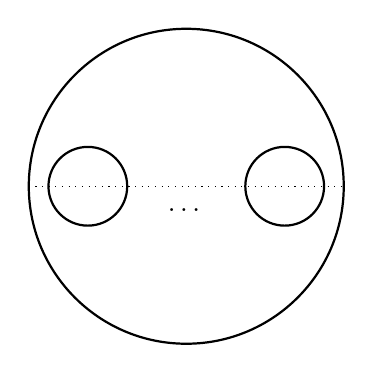
\begin{tikzpicture}
        %basepoint
        \draw[thick] (1,0) circle (2); \draw[thick] (2.25, 0) circle (0.5);
        \draw[thick] (-0.25, 0) circle (0.5);
        % \node at (-0.25, 0) {\small $1$};
        \node at (1, -0.3) {\dots};
        % \node at (2.25, 0) {\small $n$};
        \draw[dotted](-1, 0)--(3, 0);
    \end{tikzpicture}
\end{center}

Note that since $\E_2(n)$ is connected and simply connected, the quotient $\E_2
(n) \slash S_n$ is connected. Hence, it has a universal covering
$\widetilde{\E_2(n) \slash S_n}$ which we define by:
\[
    \widetilde{\E_2(n) \slash S_n} \coloneq \{ \gamma \colon [0,1] \to \E_2(n) \slash S_n \mid \gamma(0) = \bar{b}_n \} 
    \slash \text{homotopy with fixed endpoints}
\]
with projection map:
\begin{align*}
    p \colon \widetilde{\E_2(n) \slash S_n} &\to \E_2(n) \slash S_n \\
    \gamma &\mapsto \gamma(1).
\end{align*}
The topology of the covering and the fact that it defines a universal covering
of $\E_2(n) \slash S_n$ is shown in Section 1.3 in \cite{Hatcher}. Analogously,
there is a universal covering of $\E_2$, when we choose the
basepoint $b_n \in \E_2(n)$:
\begin{center}
    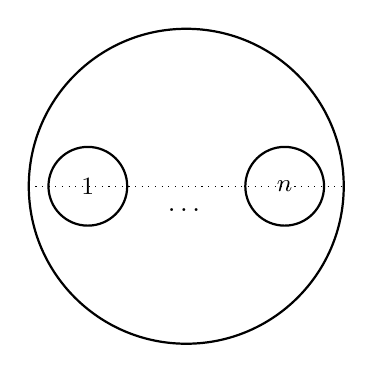
\begin{tikzpicture}
        %basepoint
        \draw[thick] (1,0) circle (2); \draw[thick] (2.25, 0) circle (0.5);
        \draw[thick] (-0.25, 0) circle (0.5); \node at (-0.25, 0) {\small $1$};
        \node at (1, -0.3) {\dots}; \node at (2.25, 0) {\small $n$};
        \draw[dotted](-1, 0)--(3, 0);
    \end{tikzpicture}
\end{center}
and define its universal covering similarly:
\[
    \widetilde{\E_2(n)} \coloneq \{ \gamma \colon [0,1] \to \E_2(n) \mid \gamma(0) = b_n \} 
    \slash \text{homotopy with fixed endpoints}
\]
with projection map:
\begin{align*}
    p \colon \widetilde{\E_2(n)} &\to \E_2(n) \\
    \gamma &\mapsto \gamma(1).
\end{align*}
There is a homeomorphism for each $n \in \N$:
\begin{align*}
    \widetilde{\E_2}(n) &\cong \widetilde{\E_2 \slash S}(n) \\
    (\gamma \colon b_n \rightsquigarrow c) &\mapsto (\bar{\gamma} \colon \bar{b}_n \rightsquigarrow \bar{c}) \\
    (\gamma \colon b_n \rightsquigarrow c') &\mapsfrom (\bar{\gamma} \colon \bar{b}_n \rightsquigarrow \bar{c}),
\end{align*}
where we forget labels in one direction and in the reverse direction we label
the basepoint $\bar{b}_n$ from left to right. The labeling of $c'$ is then
induced by the path $\gamma$. This is continuous in both directions and
inverse to one another. This shows that topologically the path $\gamma$ does not
need the labels, which is summarized in the following notation. For a path
$\gamma \colon \bar{b_n} \rightsquigarrow c$ between configurations $\bar{b_n},
c \in \widetilde{\E_2(n)} \slash S_n$ we write the following diagram in $\Ex$ for some
$\sigma \in S_n$:
\[    
    \begin{tikzcd}
        \langle n \rangle \arrow[r, "c"] \arrow[d, "\sigma"] & \langle 1 \rangle  \\
        \langle n \rangle  \arrow[r, "b_n"]                  & \langle 1 \rangle  \arrow[u, dashed, "\gamma"]              
    \end{tikzcd}
\]
Note, that the dashed arrow is not a morphism in $\Ex$ but a path of
configurations in $\E_2(n)$. Hence, the following diagram would be more
accurate, but our notation is more convenient in this section.
\begin{center}
    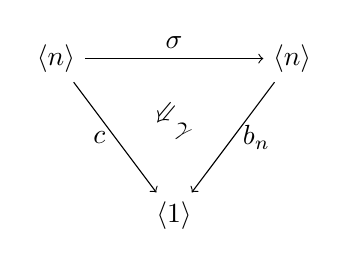
\begin{tikzpicture}
        % Define node positions
        \node (B) at (0, 2) {$\langle n \rangle$}; \node (C) at (3, 2) {$\langle
        n \rangle$}; \node (A) at (1.5, 0) {$\langle 1 \rangle$};
        
        % Draw arrows
        \draw[->] (B) -- (C) node[midway, above] {$\sigma$}; \draw[->] (B) --
        (A) node[midway, left] {$c$}; \draw[->] (C) -- (A) node[midway, right]
        {$b_n$};
        
        % Natural transformation arrow
        \node[rotate=-40] at (1.5, 1.2) {$\Downarrow \gamma$};
        % \node at (1.7, 1.2) {$\eta$};
    \end{tikzpicture}
\end{center}
Essentially, $\sigma \in S_n$ fixes the labels such that we can consider
$\gamma$ as a path in $\widetilde{\E_2}$.
\end{const}

We use this representation to define an operadic structure on
$\widetilde{\E_2} \slash S$ such that the covering is a morphism of operads and
then further use it to define a braid action on the universal covering.

First, we notice a specific translation between certain configurations that are
unique up to homotopy equivalence.

\begin{rem}[$\E_1$ translation]\label{rem:e1-translation} We observe that
    there is an embedding of $\E_1$ into $\E_2$ along the horizontal axis.

    \begin{figure}[h!]
        \begin{center}
            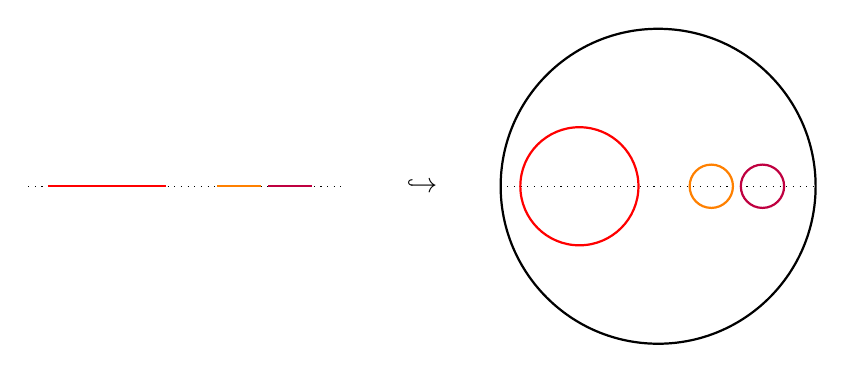
\begin{tikzpicture}
                \draw[dotted] (-13,0) -- (-9,0); \draw[thick, red] (-12.75,0) --
                (-11.25,0); \draw[thick, orange] (-10.6,0) -- (-10.05,0);
                \draw[thick, purple] (-9.95,0) -- (-9.4,0);

                % configuration in #E2
                \draw[dotted] (-7,0) -- (-3,0); \draw[thick] (-5,0) circle (2);
                \draw[thick, red] (-6, 0) circle (0.75); \draw[thick, orange]
                (-4.325, 0) circle (0.275); \draw[thick, purple] (-3.675, 0)
                circle (0.275);
                % \node at (-6.25, 0) {\small $1$}; \node at (-5, 0) {\small
                % $2$}; \node at (-3.75, 0) {\small $3$};  
                \node at (-8, 0) {$\hookrightarrow$}; 
            \end{tikzpicture}
        \end{center}
        \caption{Example of a configuration of $\E_1$ being embedded in $\E_2$
        along the horizontal line}
    \end{figure}
    Further for any $n \in \N$, two configurations $c_1, c_2 \in \E_2(n)$ that
    lie in the image of the embedding, i.e. their middle points lie on the
    horizontal axis, have a path $\eta \colon c_1 \rightsquigarrow c_2$
    corresponding to a path between the preimages in $\E_1(n$). This path is
    unique up to homotopy equivalence. This follows from the fact that the
    ordered configuration space of the real line
    \[
        \Conf_n(\R) = \left\{ (x_1, x_2, \dots, x_n) \in \mathbb{R}^n \mid x_1 < x_2 < \dots < x_n \right\}
    \]
    is contractible. We can define the following map:
    \[
    (x_1, \dots, x_n) \mapsto \left( \frac{x_2 - x_1}{x_n - x_1}, \frac{x_3 - x_1}{x_n - x_1}, \dots, \frac{x_{n-1} - x_1}{x_n - x_1} \right),
    \]
    which maps $\Conf_n(\R)$ homeomorphically onto the open standard simplex:
    \[
    \inter(\Delta^{n-2}) = \left\{ (t_1, \dots, t_{n-2}) \in (0,1)^{n-2} \mid 0 < t_1 < \dots < t_{n-2} < 1 \right\}.
    \]
    Since the open simplex $\inter(\Delta^{n-2})$ is contractible, then so is
    $\Conf_n(\R)$.
    We refer to such a unique path between two configurations in the image of
    the embedding by $\E_1$-translation. Note that this discussion holds for any
    embedding of $\E_1$ into $\E_2$.
\end{rem}

\begin{prop}
    There is an operadic structure on $\widetilde{\E_2}$ such that the covering
    $p$ is a morphism of operads.
\end{prop}

\begin{proof}
    Let 
    \[
        \gamma \colon \E_2(k) \times \E_2(j_1) \times \dots \times 
        \E_2(j_k) \to \E_2(j)
    \]
    be a composition map in $\E_2$. Then, we define a composition map in
    $\widetilde{\E_2}$
    \begin{align*}
        \widetilde{\gamma} \colon \widetilde{\E_2}(k) \times \widetilde{\E_2}(j_1) \times \dots \times 
        \widetilde{\E_2}(j_k) &\to \widetilde{\E_2}(j), \\
        % (\gamma_k, \gamma_{j_1}, \dots, \gamma_{j_k}) &\mapsto \gamma_k \circ (\gamma_{j_1}, \dots, 
        % \gamma_{j_k}) \circ \tau
    \end{align*}
    which we construct as follows: Let $(\bar{\alpha}, \alpha_1, \dots,
    \alpha_k) \in \widetilde{\E_2}(k) \times \widetilde{\E_2}(j_1) \times \dots
    \times \widetilde{\E_2}(j_k)$ with
        $$\alpha_l \colon b_{j_l} \rightsquigarrow c_l$$ for $1 \leq l \leq k$
    and 
        $$\bar{\alpha} \colon b_k \rightsquigarrow c.$$ Then 
        \[
            \bar{\alpha} \circ (\alpha_1, \dots, \alpha_k)    
        \]
    denotes the path from $\gamma(b_k, b_{j_1}, \dots, b_{j_k})$ to $\gamma(c,
    c_1, \dots, c_k)$, where we first apply

    $$\alpha_l \colon b_{j_l} \rightsquigarrow c_l$$

    on the configuration in the $l$-th disk of $b_k$ for all $1 \leq l \leq k$
    and then apply 

    $$\bar{\alpha} \colon b_k \rightsquigarrow c$$

    on the configuration $b_k$.
    \begin{figure}[h!]\label{fig:movedisks}
        
        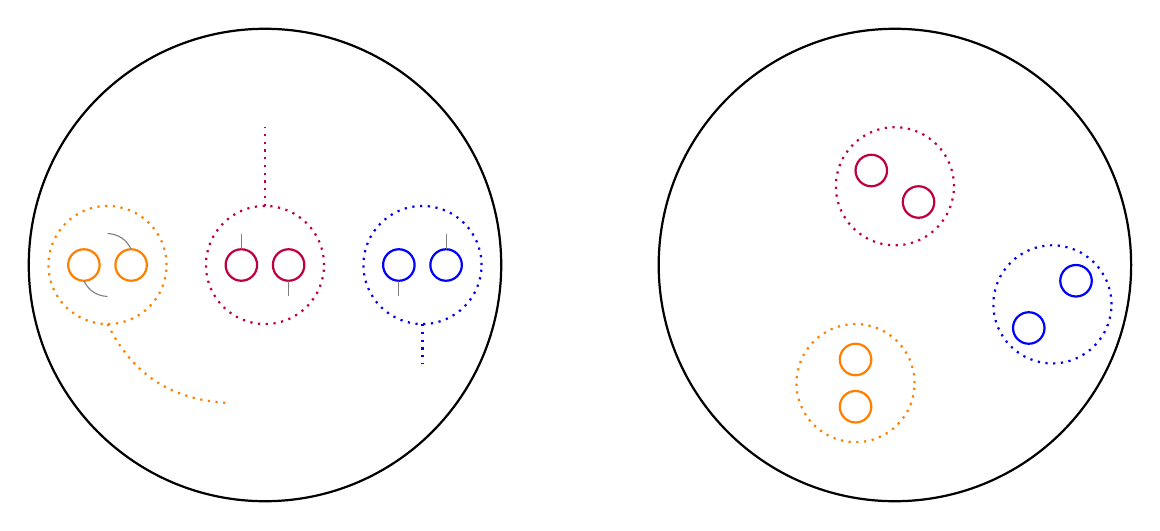
\begin{tikzpicture}
            \draw[thick] (-4,0) circle (3); \draw[dotted, thick, orange] (-6, 0)
            circle (0.75); \draw[thick, orange] (-6.3, 0) circle (0.2);
            \draw[thick, orange] (-5.7, 0) circle (0.2); \draw[dotted, thick,
            purple] (-4, 0) circle (0.75); \draw[thick, purple] (-4.3, 0) circle
            (0.2); \draw[thick, purple] (-3.7, 0) circle (0.2); \draw[dotted,
            thick, blue] (-2, 0) circle (0.75); \draw[thick, blue] (-2.3, 0)
            circle (0.2); \draw[thick, blue] (-1.7, 0) circle (0.2);

            \draw[thick] (4,0) circle (3); \draw[dotted,thick, orange] (3.5,
            -1.5) circle (0.75); \draw[thick, orange] (3.5, -1.2) circle (0.2);
            \draw[thick, orange] (3.5, -1.8) circle (0.2); \draw[dotted, thick,
            purple] (4, 1) circle (0.75); \draw[thick, purple] (3.7, 1.2) circle
            (0.2); \draw[thick, purple] (4.3, 0.8) circle (0.2);
            \draw[dotted,thick, blue] (6, -0.5) circle (0.75); \draw[thick,
            blue] (5.7, -0.8) circle (0.2); \draw[thick, blue] (6.3, -0.2)
            circle (0.2);

            %inner paths
            \draw[gray] (-6.3, -0.2) to [bend right=30] (-6, -0.4); \draw[gray]
            (-5.7, 0.2) to [bend right=30] (-6, 0.4); \draw[gray] (-4.3, 0.2) --
            (-4.3, 0.4); \draw[gray] (-3.7, -0.2) -- (-3.7, -0.4);  
            \draw[gray] (-2.3, -0.2) -- (-2.3, -0.4); \draw[gray] (-1.7, 0.2) --
            (-1.7, 0.4); 

            %outer paths to [bend right=70] (-3.75, -0.5);
            \draw[dotted, thick, orange] (-6, -0.75) to [bend right=30] (-4.5,
            -1.75); \draw[dotted, thick, purple] (-4., 0.75) -- (-4, 1.75);
            \draw[dotted, thick, blue] (-2, -0.75) -- (-2, -1.25);

            \node at (0,0) {$\rightsquigarrow$};
        \end{tikzpicture}
        \caption{Example of $\bar{\alpha} \circ (\alpha_1, \dots, \alpha_3)$ for
        $\bar{\alpha} \in \widetilde{E_2}(3)$ and $\alpha_1, \alpha_2, \alpha_3
        \in \widetilde{E_2}(2)$.}
    \end{figure}

    Further, let $\tau$ be the unique $\E_1$ translation from $b_j$ to
    $\gamma(b_k, b_{j_1}, \dots, b_{j_k})$ as discussed in Remark
    \ref{rem:e1-translation} that resizes and translates the disks along the
    horizontal axis. We obtain the following diagram:
    \begin{center}
        \begin{tikzcd}
            \langle j \rangle  \arrow[rr, "{\gamma(c, c_1, \dots, c_k)}"]
            \arrow[d, "S_j \ni"'] & & \langle 1 \rangle \\
            \langle j \rangle  \arrow[d, "S_j \ni"'] \arrow[rr, "{\gamma(b_k,
            b_{j_1}, \dots, b_{j_k})}"] & & \langle 1 \rangle  \arrow[u,
            "{\bar{\alpha} \circ (\alpha_1, \dots, \alpha_k)}"', dashed] \\
            \langle j \rangle  \arrow[rr, "b_j"] & & \langle 1 \rangle
            \arrow[u, "\tau"', dashed]                                            
        \end{tikzcd}
    \end{center}
    Therefore, we can set
    \[
        \widetilde{\gamma} (\bar{\alpha}, \alpha_1, \dots, \alpha_k) \coloneqq \bar{\alpha} \circ (\alpha_1, \dots, \alpha_k) \circ \tau.
    \]
    
    We observe that this composition map is well-defined, since the path $\tau$
    is unique up to homotopy. To see that $\widetilde{\gamma}$ is associative, we
    need to have a look at the definition. Note, that in the definition $\tau
    \in \E_1(j)$ is a path that resizes and translates the disks along the
    horizontal line. Hence, there is no braid crossing. Further, we know that composition of paths
    is associative up to homotopy. Thus, for 

    $$(\alpha, (\alpha_s)_{1 \leq s \leq k}, (\alpha_r)_{1 \leq r \leq j}) \in
    \E_2(k) \times \prod_{s=1}^{k} \E_2(j_s) \times \prod_{r=1}^{j} \E_2(i_r)$$

    we have a homotopy equivalence:
    \begin{align*}
        \left(\alpha \circ (\alpha_s)_{1 \leq s \leq k} \circ \tau^{(k)}\right) \circ \left(\alpha'_r\right)_{1 \leq r \leq j} \circ \tau^{(j)} 
        &\simeq 
        \alpha \circ \left(\alpha_s \circ (\alpha_{g_s+q})_{1 \leq q \leq j_s} \circ \tau^{(j_s)}\right)_{1 \leq s \leq k} \circ \tau^{(k)}. \\
    \end{align*}
    Furthermore, we define an operadic unit
    \[
        \eta \colon \ast \to \widetilde{\E_2(1)}
    \]
    to be the trivial path of the trivial basepoint $\id^{(1)} \in \E_2(1)$. Clearly,
    this unit fulfills the unitality conditions.

    Finally, we need to show that the covering map $p \colon \widetilde{\E_2}\to
    \E_2$ is a morphism of operads. For this, we need to convince ourselves that
    the following diagram commutes for all $n \geq 1$:
    \begin{center}
        \begin{tikzcd}
            \widetilde{\E_2(k)} \times \widetilde{\E_2(j_1)} \times \dots \times
            \widetilde{\E_2(j_k)} \arrow[d, "\widetilde{\gamma}"] \arrow[rr,
            "p"] &  & \E_2(k)\times \E_2(j_1) \times \dots \times \E_2(j_k)
            \arrow[d, "\gamma"] \\
            \widetilde{\E_2(j)} \arrow[rr, "p"] &  & \E_2(j)                                                                                             
        \end{tikzcd}
    \end{center}
    This is indeed the case, by definition of $\widetilde{\gamma}$ we have:
    \[
        p \circ \widetilde{\gamma} (\bar{\alpha}, \alpha_1, \dots, \alpha_k) = \gamma(c, c_1, \dots, c_k)
    \]
    for $\alpha_l \colon b_{j_l} \to c_l$ for $1 \leq l \leq k$ and
    $\bar{\alpha} \colon b_k \to c$. The unitality condition is also
    met by definition:
    \begin{center}
        \begin{tikzcd}
                                        & \ast \arrow[ld, "\widetilde{\eta}"']
                                        \arrow[rd, "\eta"] & \\
            \widetilde{\E_2}(1) \arrow[rr, "p"] & & \E_2(1)
        \end{tikzcd}
    \end{center}
    This concludes the proof that $\widetilde{\E_2}$ admits an operadic
    structure and that the covering map is a morphism of operads.
\end{proof}

\begin{rem}
    This construction of an operadic structure on the universal covering of a
    topological operad can be given in a more general setting, which we do not
    require at this point. But in \cite[Lemma 4.1.12]{adrian} one can find a
    more general statement on how to construct an operadic structure on the
    collection of level-wise universal coverings of a sufficiently connected
    topological operad as long as there is a suboperad of $\E_1$ contained in the
    topological operad.
\end{rem}
   
\begin{const}[Braid Action on $\widetilde{\E_2 \slash S}$]
We want to define a braid action on the universal covering $\widetilde{\E_2}$.
As we have seen previously, the universal covering of $\E_2 \slash S$ is
level-wise homeomorphic to the universal covering of $\E_2$. As usual, there is
a group action of the fundamental group of $\E_2(n) \slash S(n)$ on its
universal covering. By Lemma \ref{lem:fundamentalgroup} the fundamental group of $\E_2(n)$ is the $n$-th pure braid
group $PB_n$. But since we forgot the labels when moving to $\E_2(n) \slash
S(n)$, we now obtain the full $n$-th braid group $B_n$. Since there is a
homeomorphism $\widetilde{\E_2 \slash S} \cong \widetilde{\E_2}$, we can lift
the braid group action to $\widetilde{\E_2}$. For a detailed proof, we refer to
the paper of Fox and Neuwirth \cite{fox}. However, we give a short overview of
the construction here.

We recall the generators of $B_n$ for all $1 \leq i < n$, $n \in \N$:
\begin{center}
    \begin{tikzpicture}
        \pic[ braid/number of strands=6, braid/strand 2/.style={white},
        braid/strand 5/.style={white}, name=coordinates, ] at (0,0)
        {braid={s_3}}; \node[at=(coordinates-rev-2-e)] {$\dots$};
        \node[at=(coordinates-rev-3-e), below=3pt] {$i$};
        \node[at=(coordinates-rev-4-e), below=3pt] {$i+1$};
        \node[at=(coordinates-rev-5-e)] {$\dots$}; \node[anchor=center] at
        (-0.5,-0.75) {$\sigma_i = \quad $};
    \end{tikzpicture}
\end{center}

We identify the generators with the homotopy class of the half twist of the
$i$-th and $(i+1)$-th disk in $\widetilde{\E_2 \slash S}$, which we also
denote by $\sigma_i$ from now on:
\begin{center}
    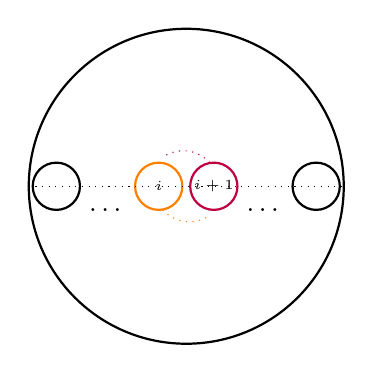
\begin{tikzpicture}
        %basepoint
        \draw[thick] (0,0) circle (2); \draw[thick] (1.65, 0) circle (0.3);
        \draw[thick, purple] (0.35, 0) circle (0.3); \draw[thick, orange]
        (-0.35, 0) circle (0.3); \draw[thick] (-1.65, 0) circle (0.3);
        % \node at (-0.25, 0) {\small $1$};
        \node at (1., -0.3) {\dots}; \node at (-1., -0.3) {\dots}; \node at
        (0.35, 0) {\tiny{$i+1$}}; \node at (-0.35, 0) {\tiny{$i$}};

        \draw[dotted, purple](0.3, 0.3) [bend right=40] to (-0.3, 0.37);
        \draw[dotted, orange](-0.3, -0.3) [bend right=40] to (0.3, -0.37);
        \draw[dotted](-2, 0)--(2, 0);
    \end{tikzpicture}
\end{center}

Then, we obtain a braid action on $\widetilde{\E_2}$. Let $\alpha \colon b_n \to
c$ be in $\widetilde{\E_2 \slash S}$, which is represented by the following
diagram in $\Ex$ for some $\tau \in S_n$:

\begin{center}
    \begin{tikzcd}
        \langle n \rangle \arrow[r, "c"] \arrow[d, "\tau"']         & \langle 1
        \rangle                                   \\
        \langle n \rangle \arrow[r, "b_n"] & \langle 1 \rangle \arrow[u,
        "\alpha"', dashed]
    \end{tikzcd}
\end{center}

Let $\sigma \in B_n$, then we set:
\[
    \sigma . \alpha \coloneq \alpha \circ \sigma^{-1}.
\]

Concatenating these paths results in the following commuting diagram, where
$\bar{\sigma} \in S_n$ refers to the underlying permutation of $\sigma$.

\begin{center}
    \begin{tikzcd}
        \langle n \rangle \arrow[r, "c"] \arrow[d, "\tau"']         & \langle 1
        \rangle                                   \\
        \langle n \rangle \arrow[d, "\bar{\sigma}"'] \arrow[r, "b_n"] & \langle
        1 \rangle \arrow[u, "\alpha"', dashed]      \\
        \langle n \rangle \arrow[r, "b_n"]                            & \langle
        1 \rangle \arrow[u, "\sigma^{-1}"', dashed]
    \end{tikzcd}
\end{center}

It is left to show that this braid action is equivariant with respect to
the operadic structure on $\widetilde{\E_2}$. Note that by
definition of $\widetilde{\gamma}$ we move disks in a large disk $D$ from the
basepoint configuration to another configuration once and afterwards we do not touch the
configuration of $D$ again but only move $D$ as a disk of another
configuration.
Hence, in that sense the order in which we apply paths to a
configuration does not matter from a homotopy perspective. This fact is
equivalent to the fact that we can pull inside braids through outside braids,
i.e. the second relation of braids in Remark \ref{braidgrouprem}:
\begin{center}
    \begin{tikzpicture}
        \pic[ braid/number of strands=7, braid/strand 4/.style={white},
        name=coordinates, ] at (0,0) {braid={s_1-s_6 s_2-s_5 s_1-s_6}};
        
        \node[at=(coordinates-rev-1-e), below=3pt] {$i$};
        \node[at=(coordinates-rev-2-e), below=3pt] {$i+1$};
        \node[at=(coordinates-rev-3-e), below=3pt] {$i+2$};
        \node[at=(coordinates-rev-5-e), below=3pt] {$i$};
        \node[at=(coordinates-rev-6-e), below=3pt] {$i+1$};
        \node[at=(coordinates-rev-7-e), below=3pt] {$i+2$};
    
        \node[anchor=center] at (3,-1.8) {$=$};
    \end{tikzpicture}
\end{center}
This means that for all $\sigma \in B_k$, we have the following commutative
diagram:

\begin{center}
    \begin{tikzcd}
    \widetilde{\E_2}(k) \times \widetilde{\E_2}(j_1) \times \dots \times
    \widetilde{\E_2}(j_k) \arrow[d, "\widetilde{\gamma}"] \arrow[rr, "\sigma
    \times \bar{\sigma}"] &  & \widetilde{\E_2}(k) \times
    \widetilde{\E_2}(j_{\bar{\sigma}(1)}) \times \dots \times
    \widetilde{\E_2}(j_{\bar{\sigma}(k)}) \arrow[d, "\widetilde{\gamma}"] \\
    \widetilde{\E_2}(j) \arrow[rr, "{\sigma(j_1, \dots, j_k)}"] &  &
    \widetilde{\E_2}(j)                                                                                                       
    \end{tikzcd}
\end{center}

and for $\tau_i \in B_{j_i}$ with $1 \leq i \leq k$, we have the following
commutative diagram:
\begin{center}
    \begin{tikzcd}
    \widetilde{\E_2}(k) \times \widetilde{\E_2}(j_1) \times \dots \times
    \widetilde{\E_2}(j_k) \arrow[d, "\widetilde{\gamma}"] \arrow[rr, "{(\id,
    \tau_1, \dots, \tau_k)}"] &  & \widetilde{\E_2}(k) \times
    \widetilde{\E_2}(j_1) \times \dots \times \widetilde{\E_2}(j_k) \arrow[d,
    "\widetilde{\gamma}"] \\
    \widetilde{\E_2}(j) \arrow[rr, "\tau_1 \oplus \dots \oplus \tau_k"] &  &
    \widetilde{\E_2}(j)                                                                                                       
    \end{tikzcd}
\end{center}

Hence, the braid group action on $\widetilde{\E_2}$ respects the operadic
structure.

\end{const}